\documentclass{article}
\usepackage[utf8x]{inputenc}
\usepackage{graphicx}
\usepackage{amsmath}
\usepackage{amssymb}
\usepackage{tikz}
\usepackage{todonotes}
\usepackage{pgfplots}
\usepackage{epstopdf}
\usepackage{listings}
\usepackage{circuitikz}
\usepackage{float}
\usepackage{cleveref}
\usepackage{ragged2e} % For text alignment


\newenvironment{custom_itemize}{
\begin{itemize}
  \setlength{\itemsep}{0pt}
  \setlength{\parskip}{0pt}
  \setlength{\parsep}{0pt}
}{\end{itemize}}


\usepackage[hmarginratio=1:1,top=22mm,columnsep=16pt]{geometry} % Document margins
%\usepackage{multicol} % Used for the two-column layout of the document


%\usepackage{bm}


\title{Preethis ROIC analysis}
\author{Kees Kroep 4246373}


\begin{document}
%  \twocolumn[{%
% \begin{@twocolumnfalse}
  \maketitle
%   \end{@twocolumnfalse}
% }]

\section{setup}\label{sec:setup}

\begin{figure}[h]
	\centering
	\includegraphics[width=0.6\linewidth]{fig/setup_overview.eps}
	\caption{setup overview}
	\label{fig:setup_overview}
\end{figure}

\begin{figure}[h]
	\centering
	\includegraphics[width=0.6\linewidth]{fig/close-up.eps}
	\caption{close-up}
	\label{fig:close-up}
\end{figure}

\clearpage
\section{grounded versus floating}
This test addresses the effect of a grounded input versus a floating input. Rst1=Rst2=0.
The behavior of the floating channel changes dramatically based on the voltage used to power $VDD\_HV$. When the input is grounded, the output is not affected by the voltage on the VDD\_HV. This is illustrated below.

\begin{figure}[H]
	\centering
	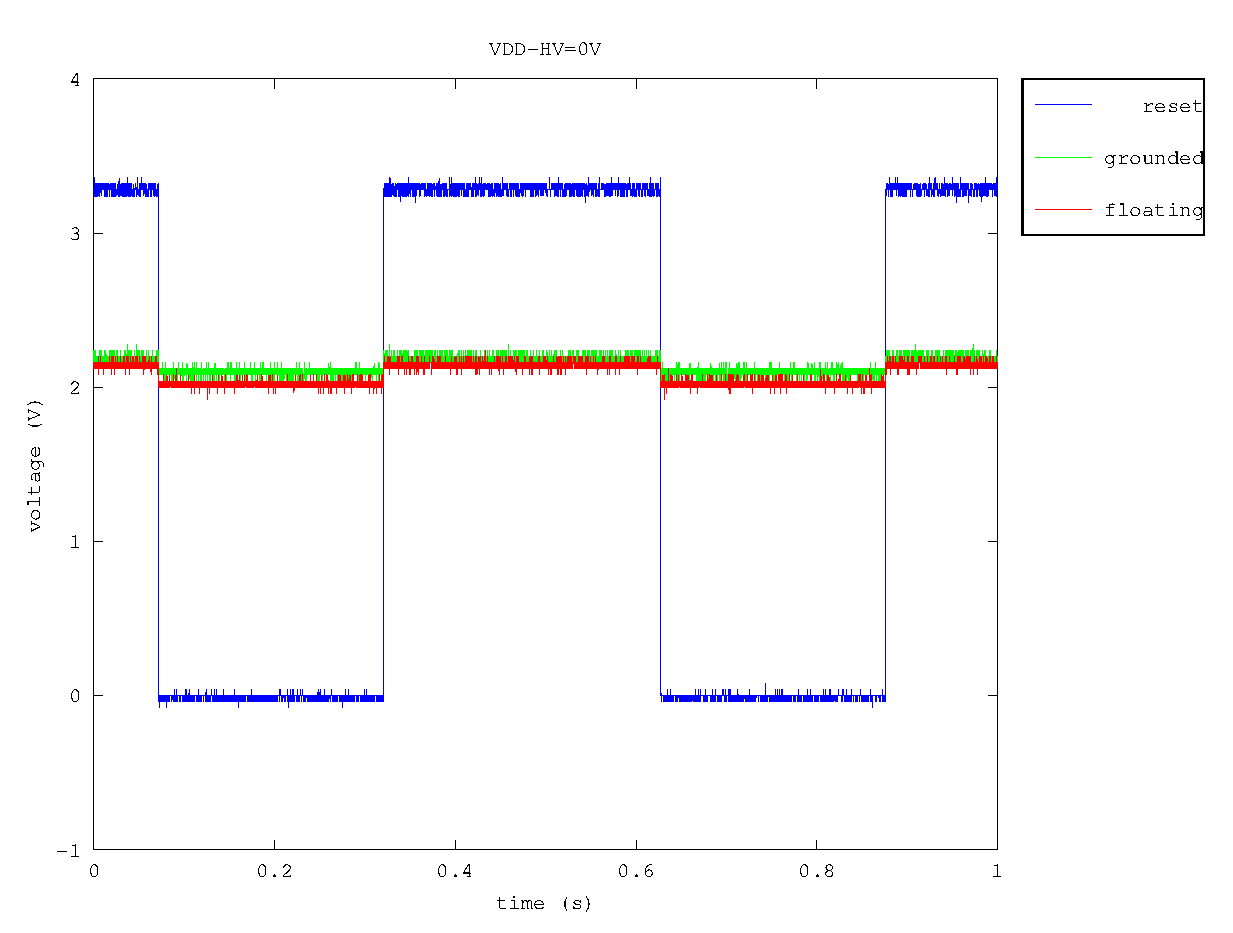
\includegraphics[width=0.8\linewidth]{fig/g_f_0V.eps}
	\caption{floating versus grounded. $VDD\_HV=0\,V$}
	\label{fig:g_f_0V}
\end{figure}

\begin{figure}[H]
	\centering
	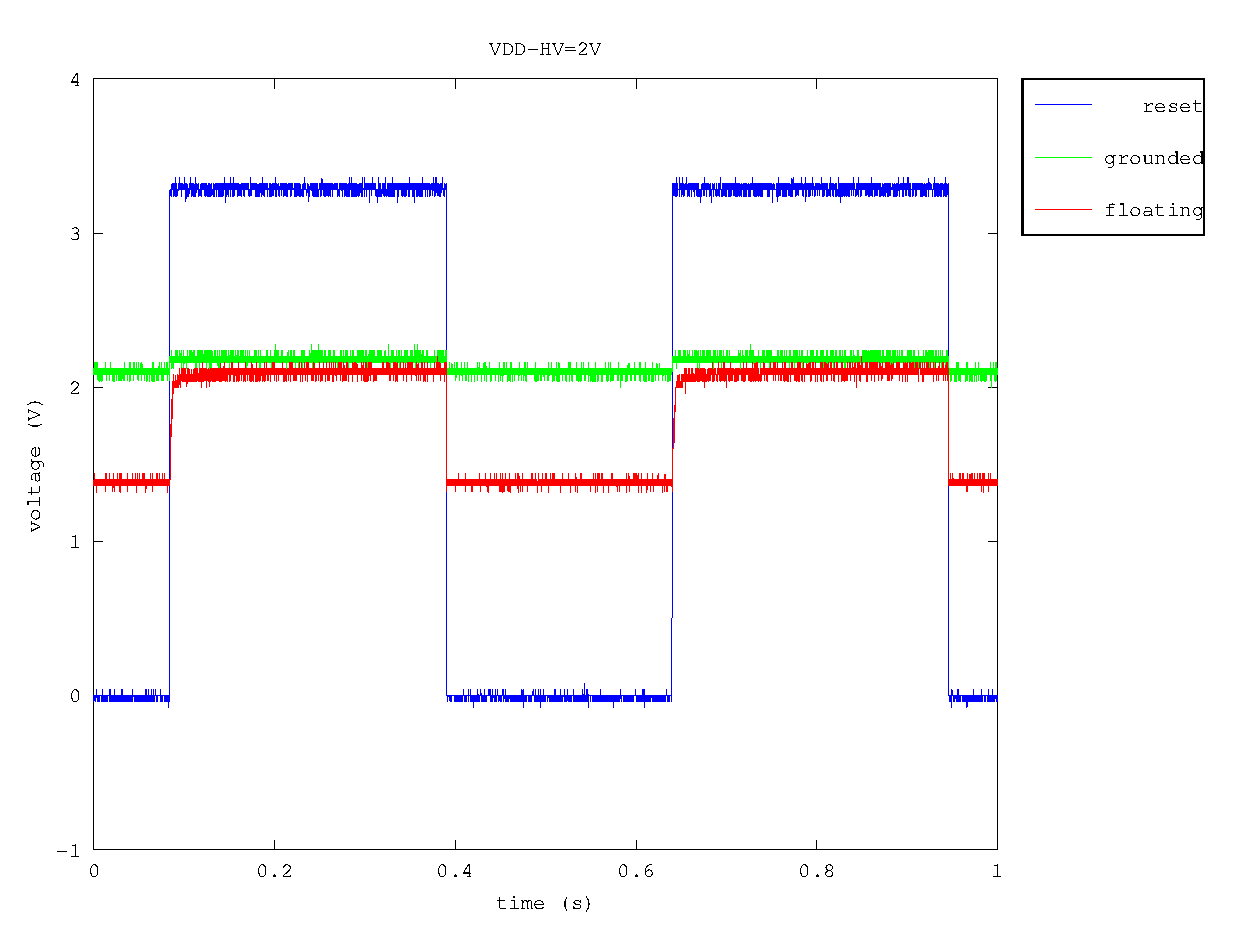
\includegraphics[width=0.8\linewidth]{fig/g_f_2V.eps}
	\caption{floating versus grounded. $VDD\_HV=2\,V$}
	\label{fig:g_f_2V}
\end{figure}

\begin{figure}[H]
	\centering
	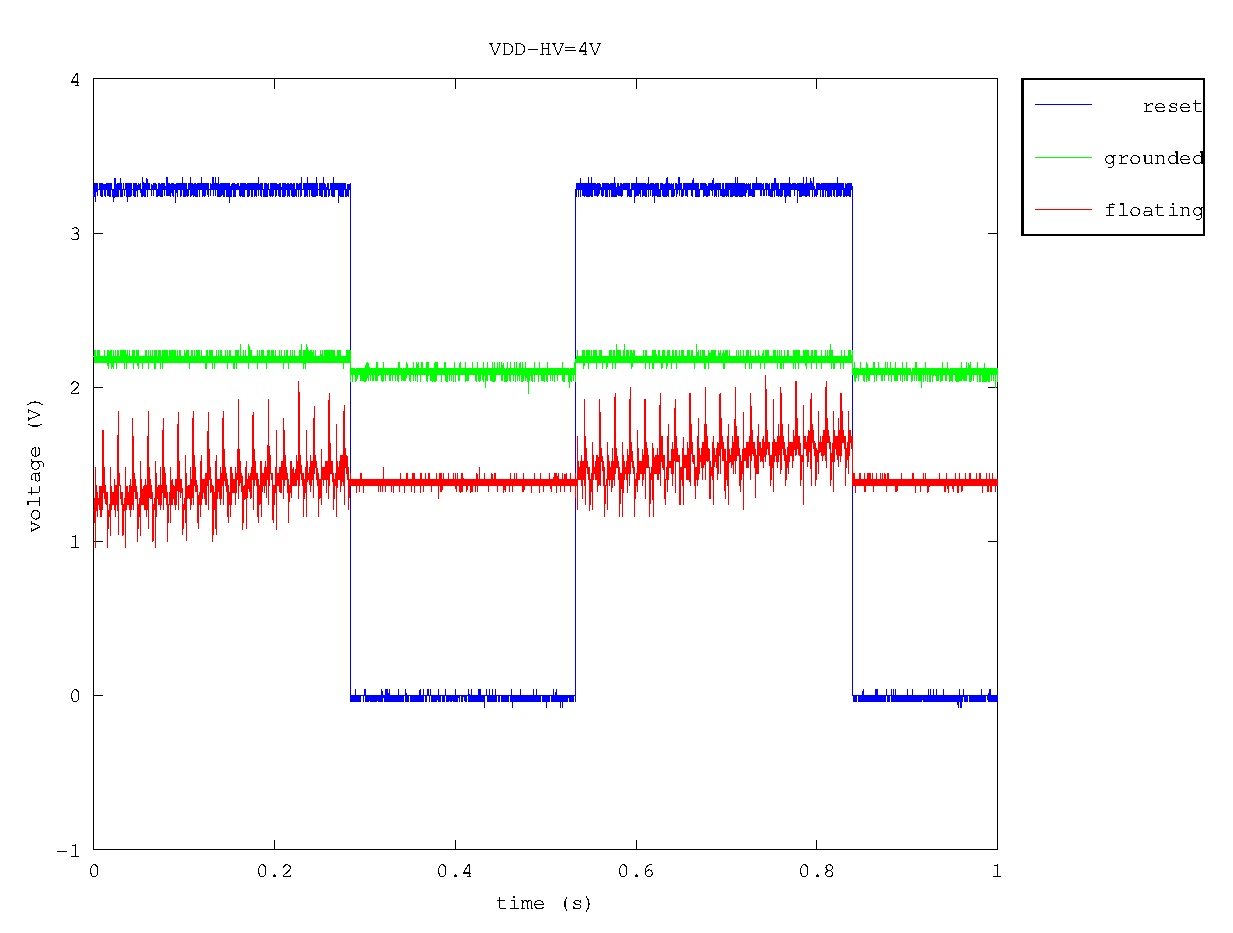
\includegraphics[width=0.8\linewidth]{fig/g_f_4V.eps}
	\caption{floating versus grounded. $VDD\_HV=4\,V$}
	\label{fig:g_f_4V}
\end{figure}

\begin{figure}[H]
	\centering
	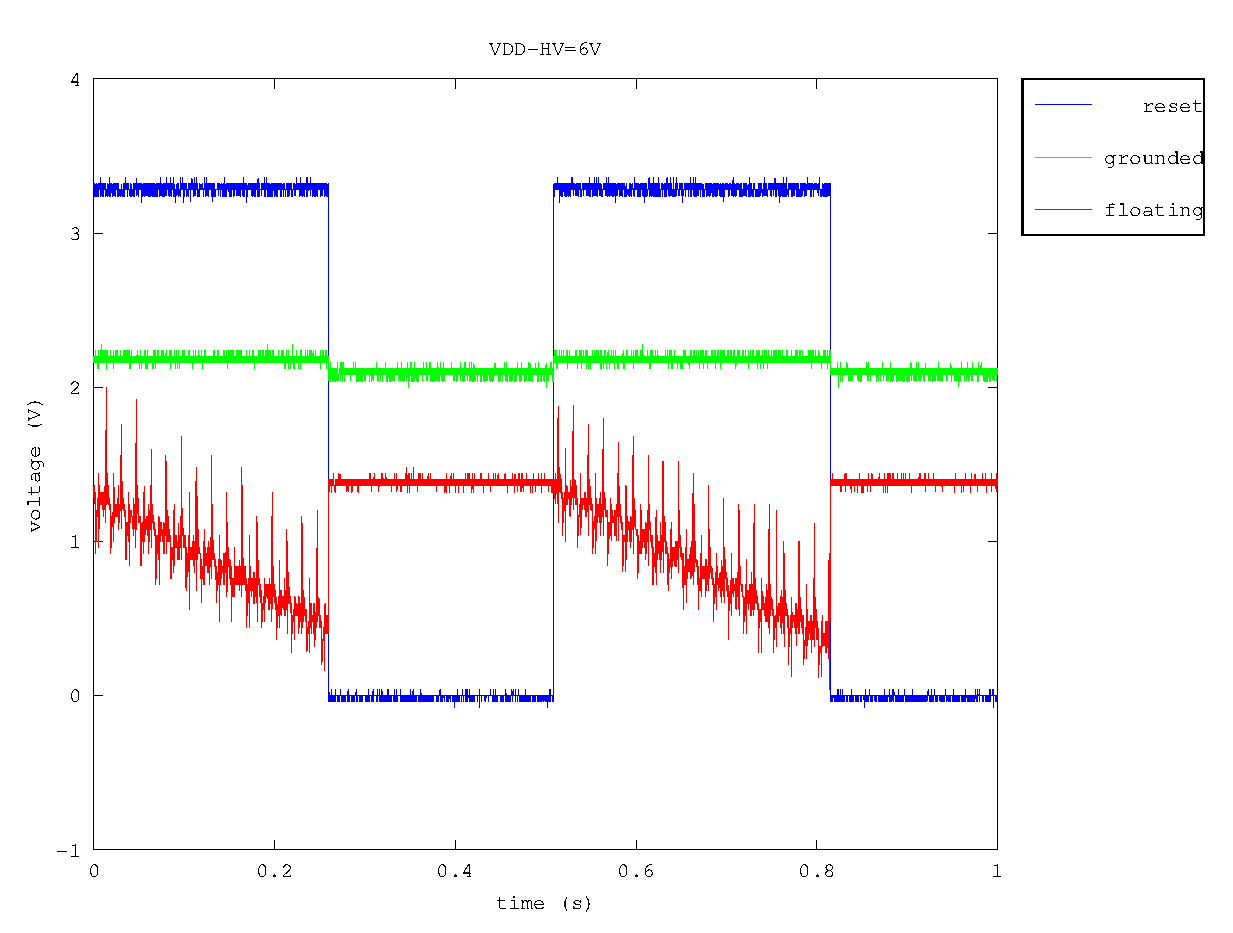
\includegraphics[width=0.8\linewidth]{fig/g_f_6V.eps}
	\caption{floating versus grounded. $VDD\_HV=6\,V$}
	\label{fig:g_f_6V}
\end{figure}

\begin{figure}[H]
	\centering
	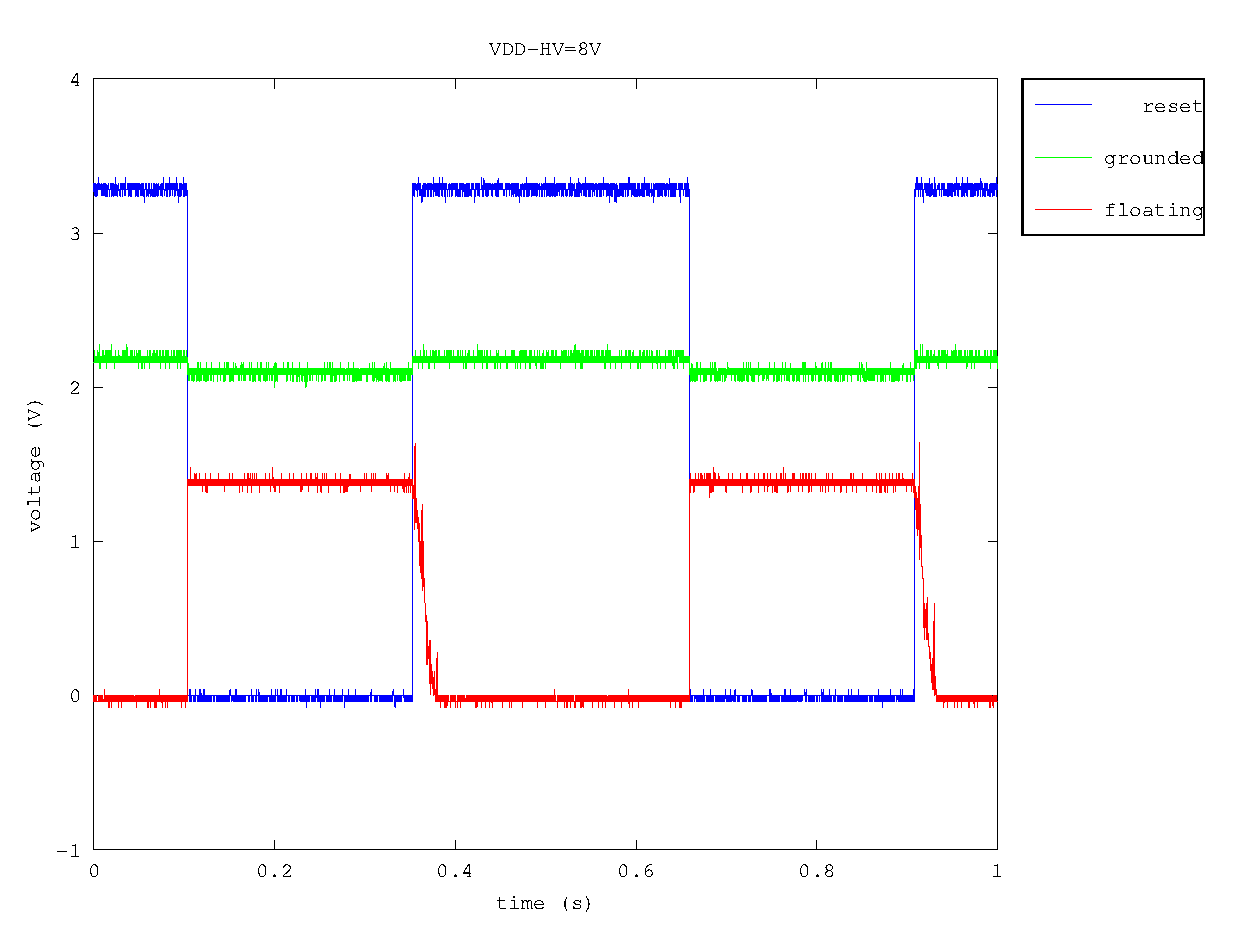
\includegraphics[width=0.8\linewidth]{fig/g_f_8V.eps}
	\caption{floating versus grounded. $VDD\_HV=8\,V$}
	\label{fig:g_f_8V}
\end{figure}

\begin{figure}[H]
	\centering
	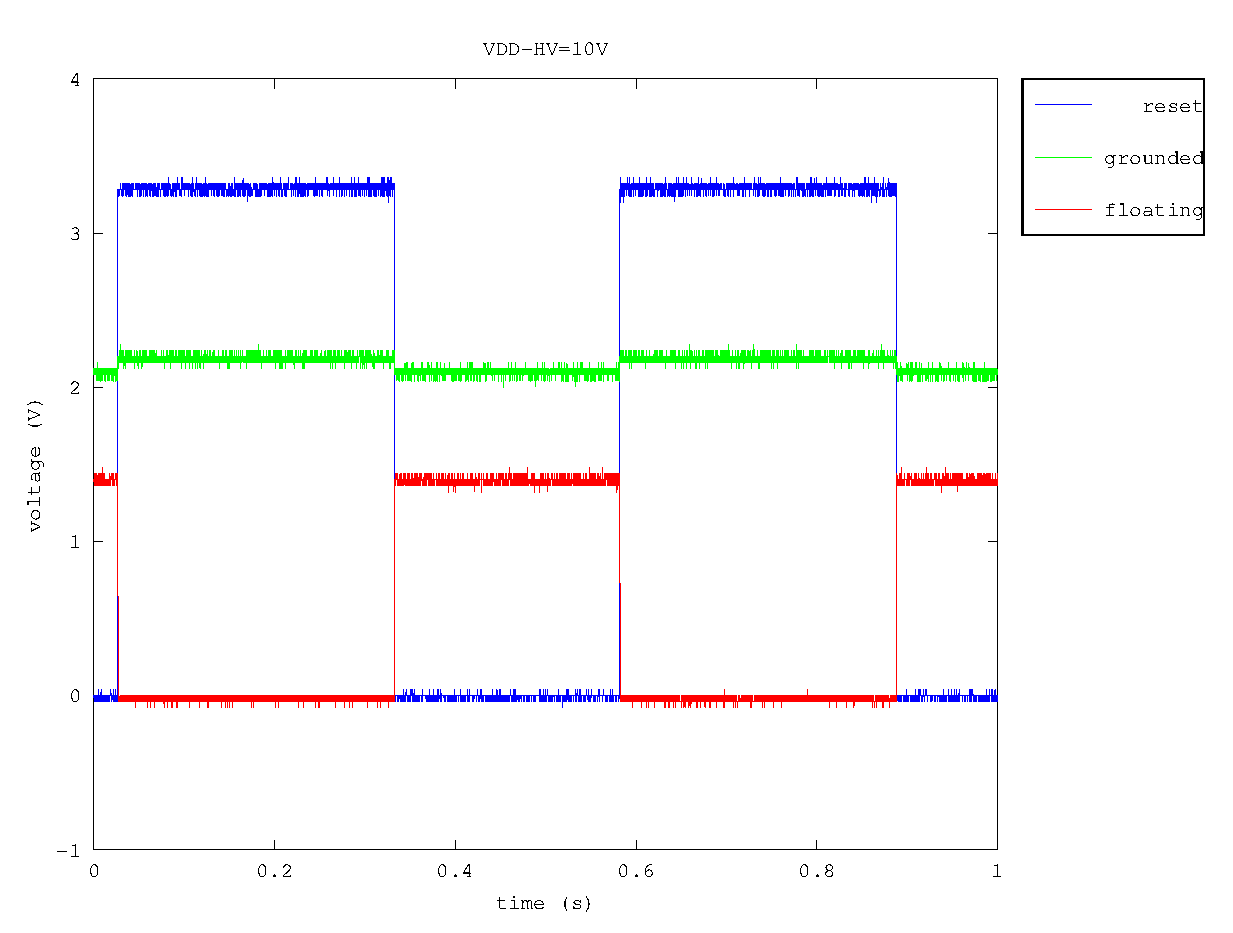
\includegraphics[width=0.8\linewidth]{fig/g_f_10V.eps}
	\caption{floating versus grounded. $VDD\_HV=10\,V$}
	\label{fig:g_f_10V}
\end{figure}

\section{input vs output}
This test addresses the relationship between input and output. Rst1=Rst2=0 V. The input is a voltage source in series with a transistor of $20\,M\Omega$. The VDD\_HV = $4.5\,V$. In this particular set-up the relationship between the input and output does not behave as (I) expected. There is no difference in performance for the input voltage $<2.2\,V$ and $>2.6\,V$. The performance of the input voltage between $2.2$ and $2.6\,V$ are shown below. 

\begin{figure}[H]
	\centering
	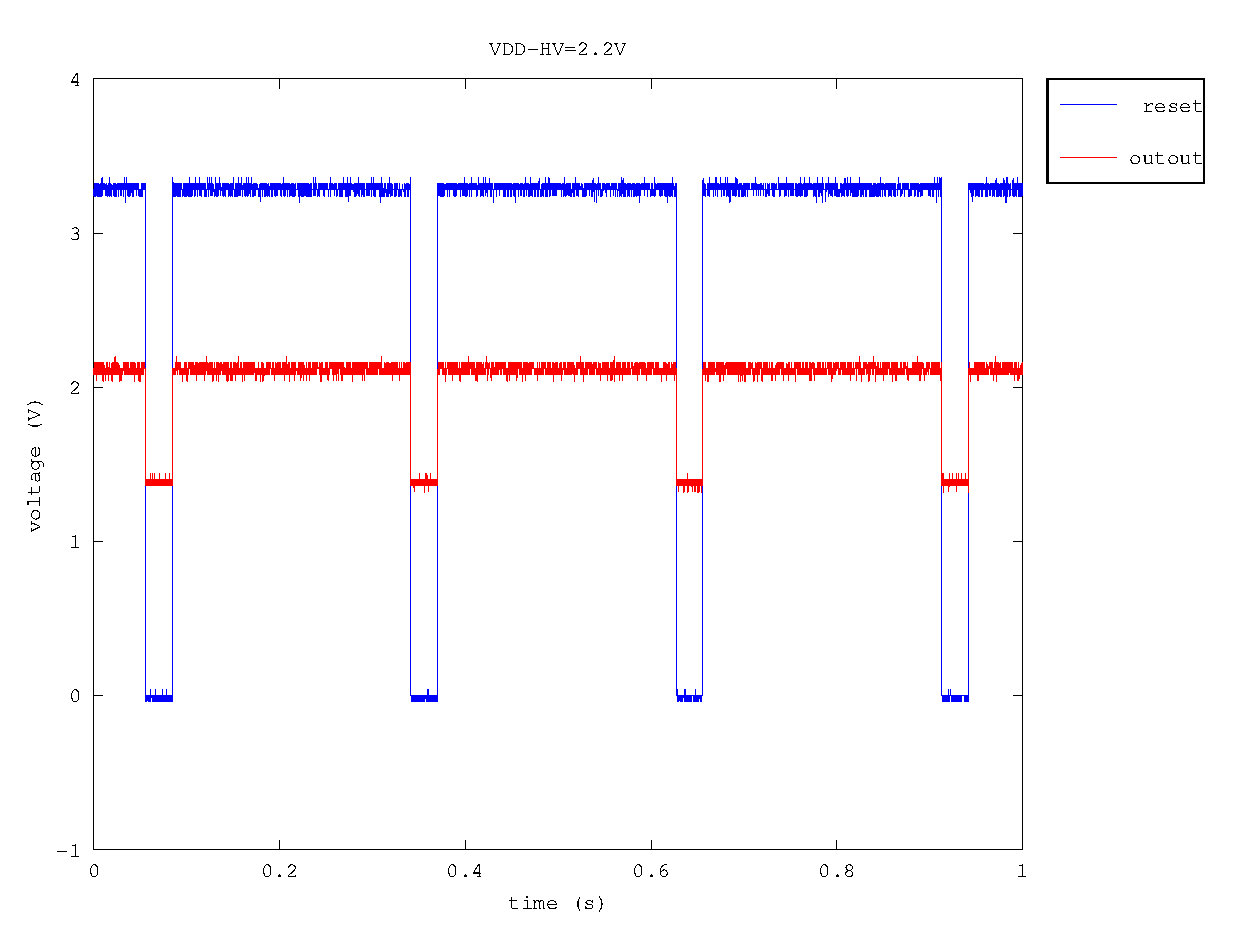
\includegraphics[width=0.8\linewidth]{fig/out_2-2V.eps}
	\caption{output of channel with constant input current. $VDD\_HV=2.2\,V$}
	\label{fig:out_2-2V}
\end{figure}

\begin{figure}[H]
	\centering
	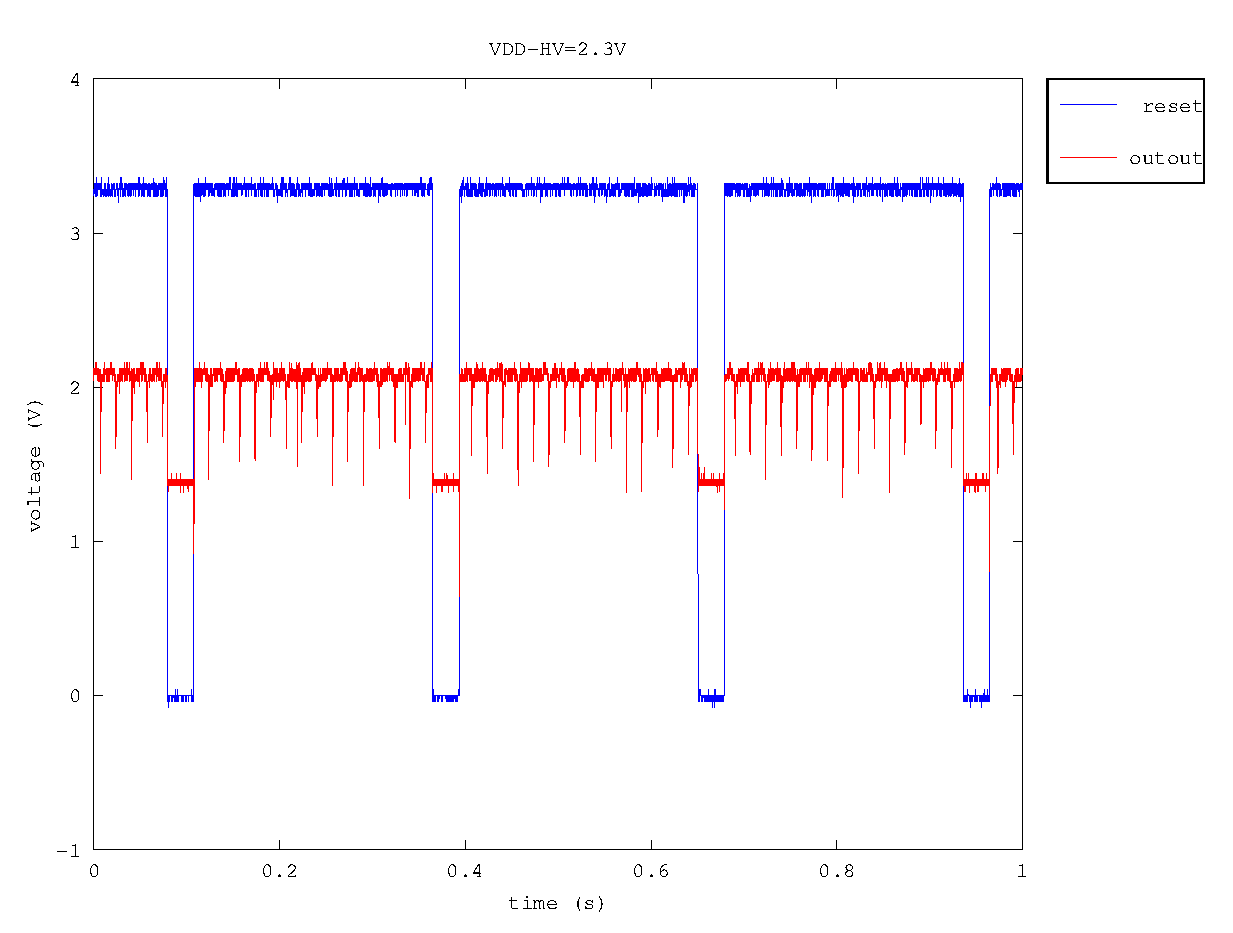
\includegraphics[width=0.8\linewidth]{fig/out_2-3V.eps}
	\caption{output of channel with constant input current. $VDD\_HV=2.3\,V$}
	\label{fig:out_2-3V}
\end{figure}

\begin{figure}[H]
	\centering
	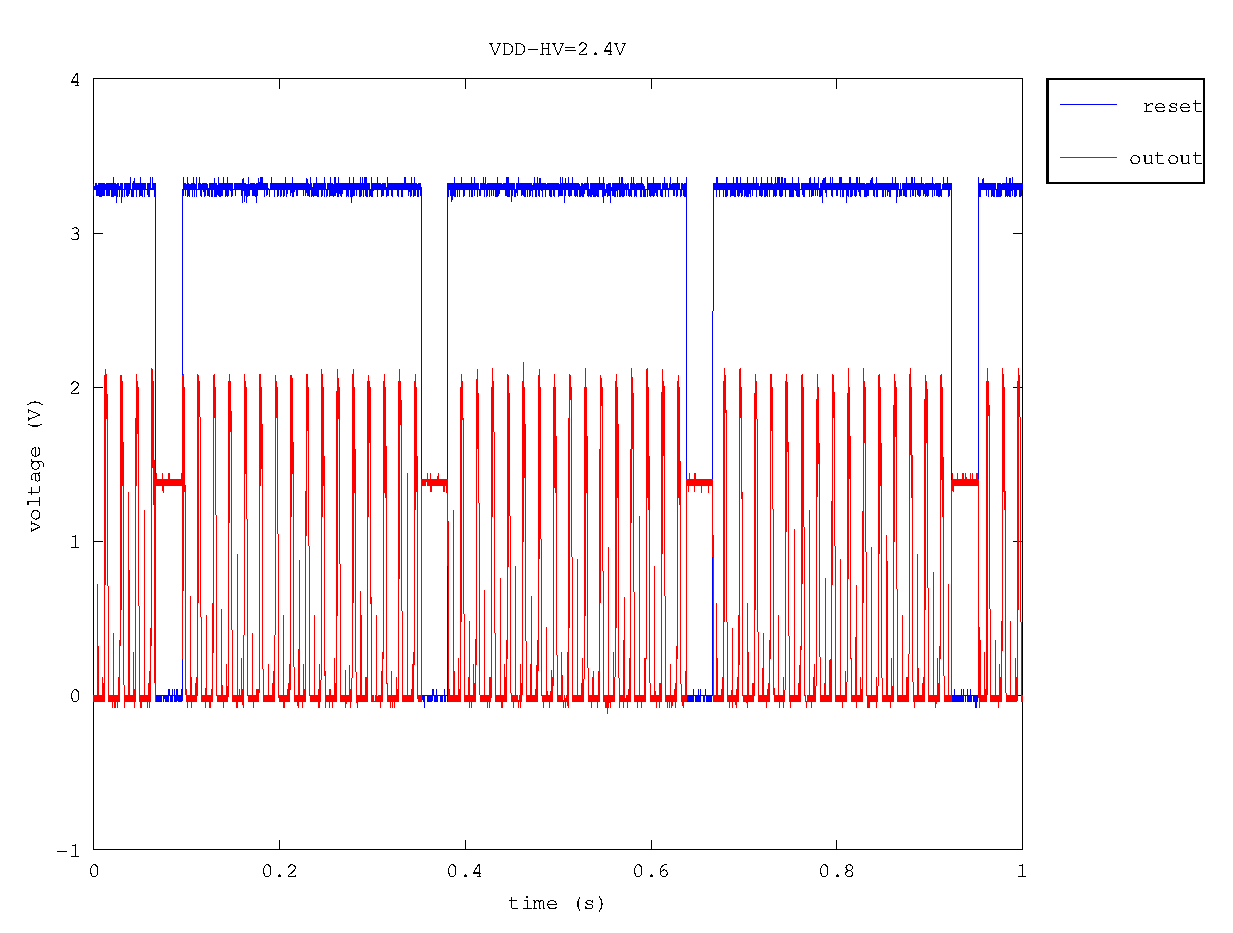
\includegraphics[width=0.8\linewidth]{fig/out_2-4V.eps}
	\caption{output of channel with constant input current. $VDD\_HV=2.4\,V$}
	\label{fig:out_2-4V}
\end{figure}

\begin{figure}[H]
	\centering
	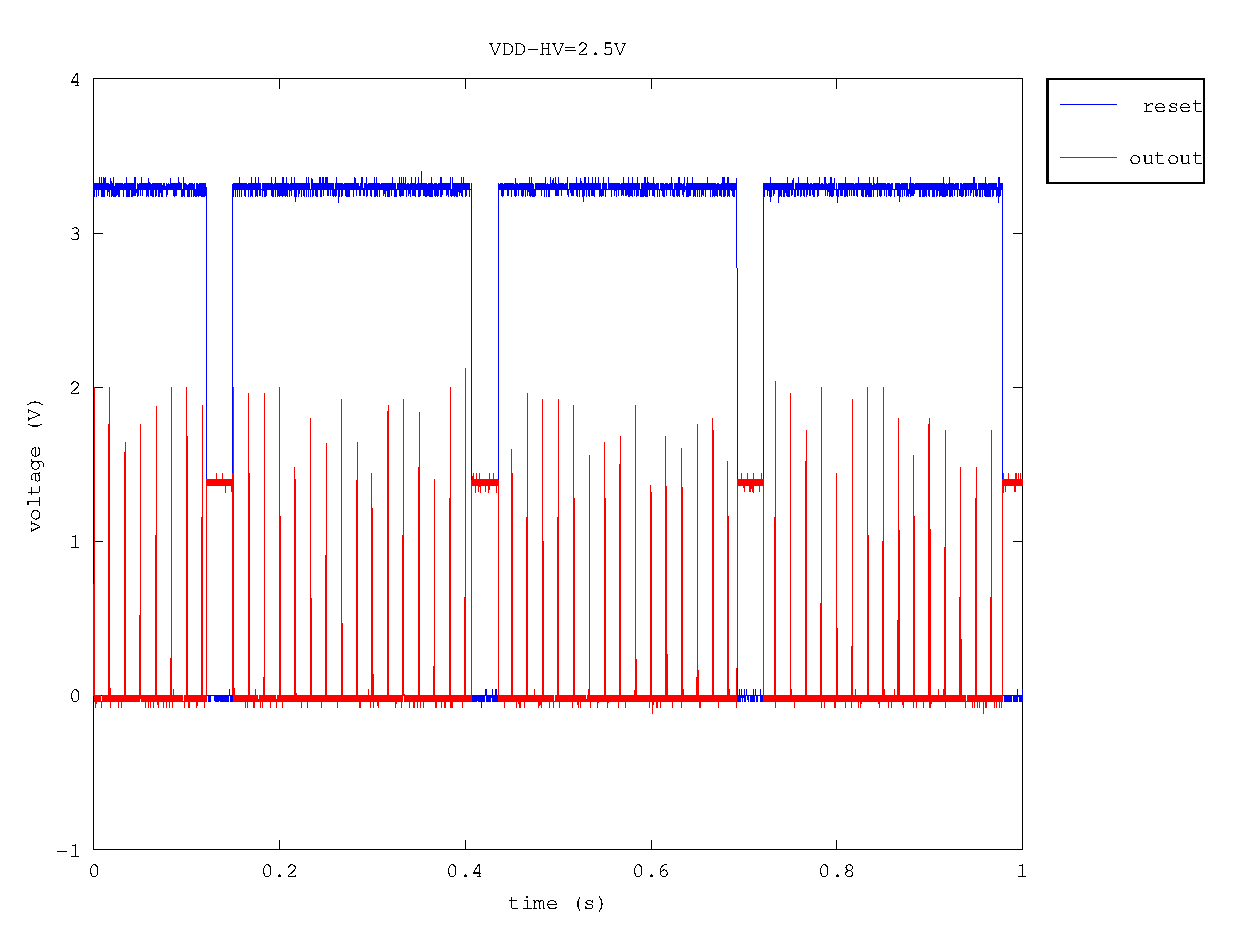
\includegraphics[width=0.8\linewidth]{fig/out_2-5V.eps}
	\caption{output of channel with constant input current. $VDD\_HV=2.5\,V$}
	\label{fig:out_2-5V}
\end{figure}



\begin{figure}[H]
	\centering
	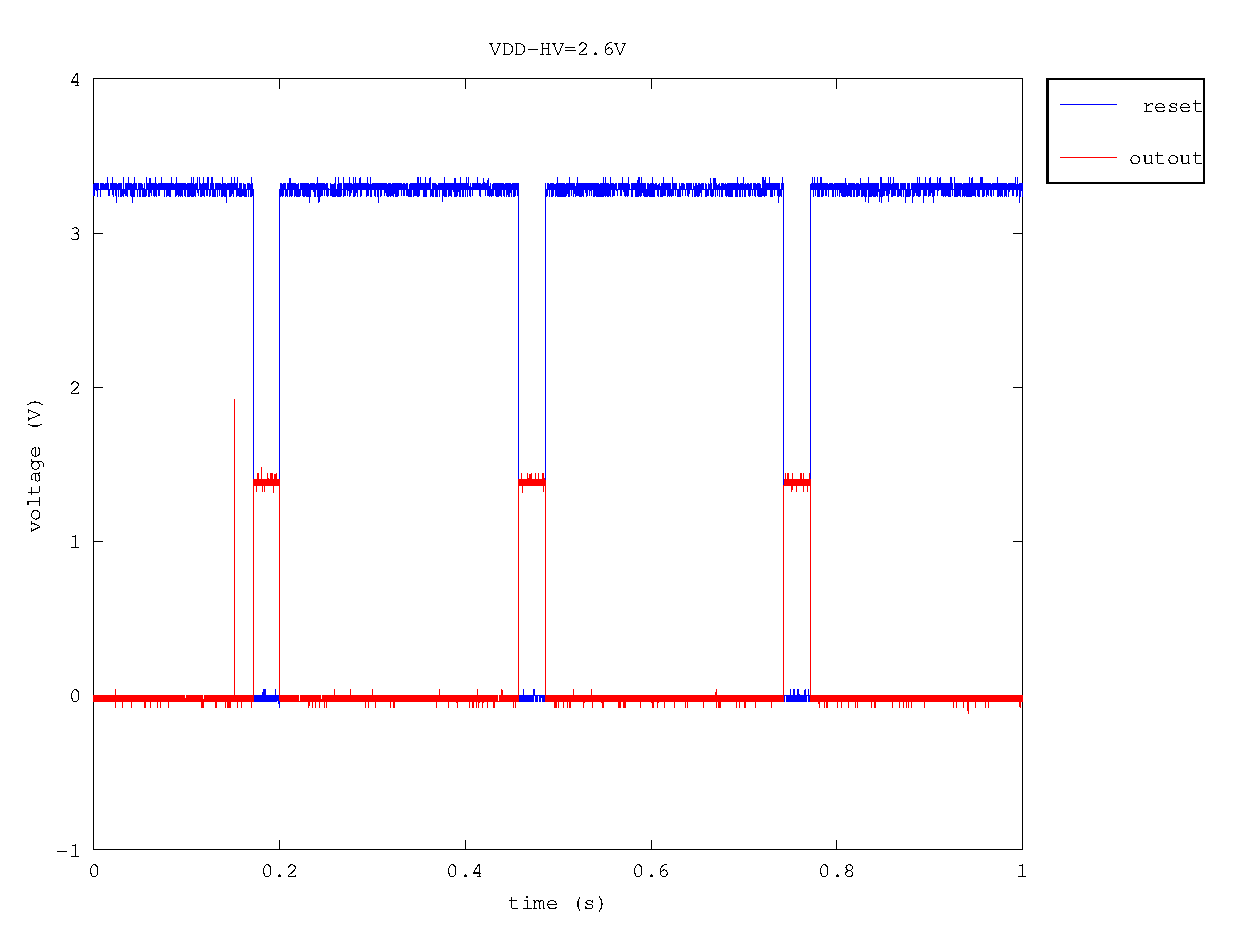
\includegraphics[width=0.8\linewidth]{fig/out_2-6V.eps}
	\caption{output of channel with constant input current. $VDD\_HV=2.6\,V$}
	\label{fig:out_2-6V}
\end{figure}

\section{VB}
This test addresses the effect of the voltage limiter. Both the output and VB of a channel are observed under varying input voltages. The test results show that the VB rises to approximately $2\,V$ and then stops rising.

\begin{figure}[H]
	\centering
	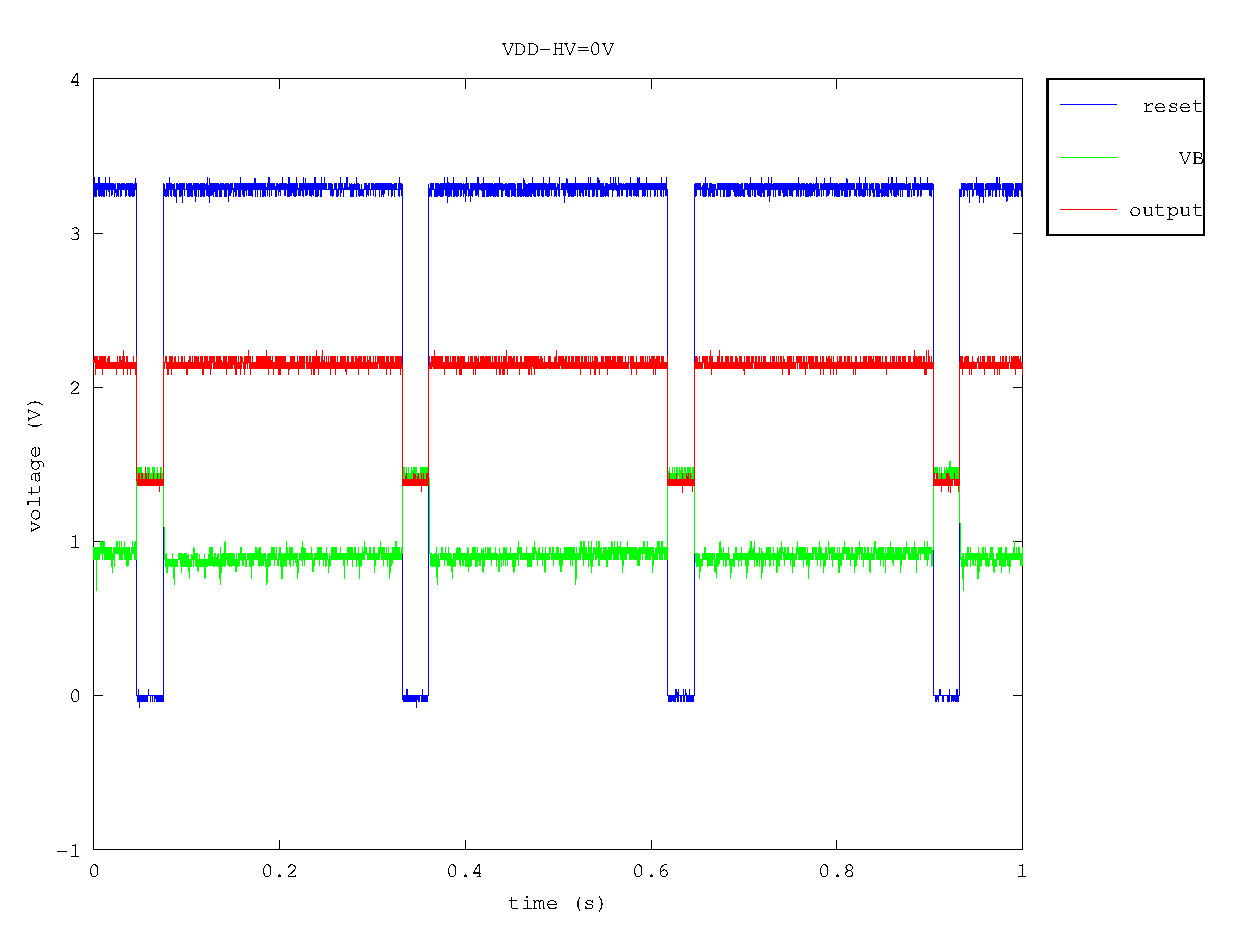
\includegraphics[width=0.8\linewidth]{fig/VB_0V.eps}
	\caption{VB and output for $VDD\_HV=0\,V$}
	\label{fig:VB_0V}
\end{figure}

\begin{figure}[H]
	\centering
	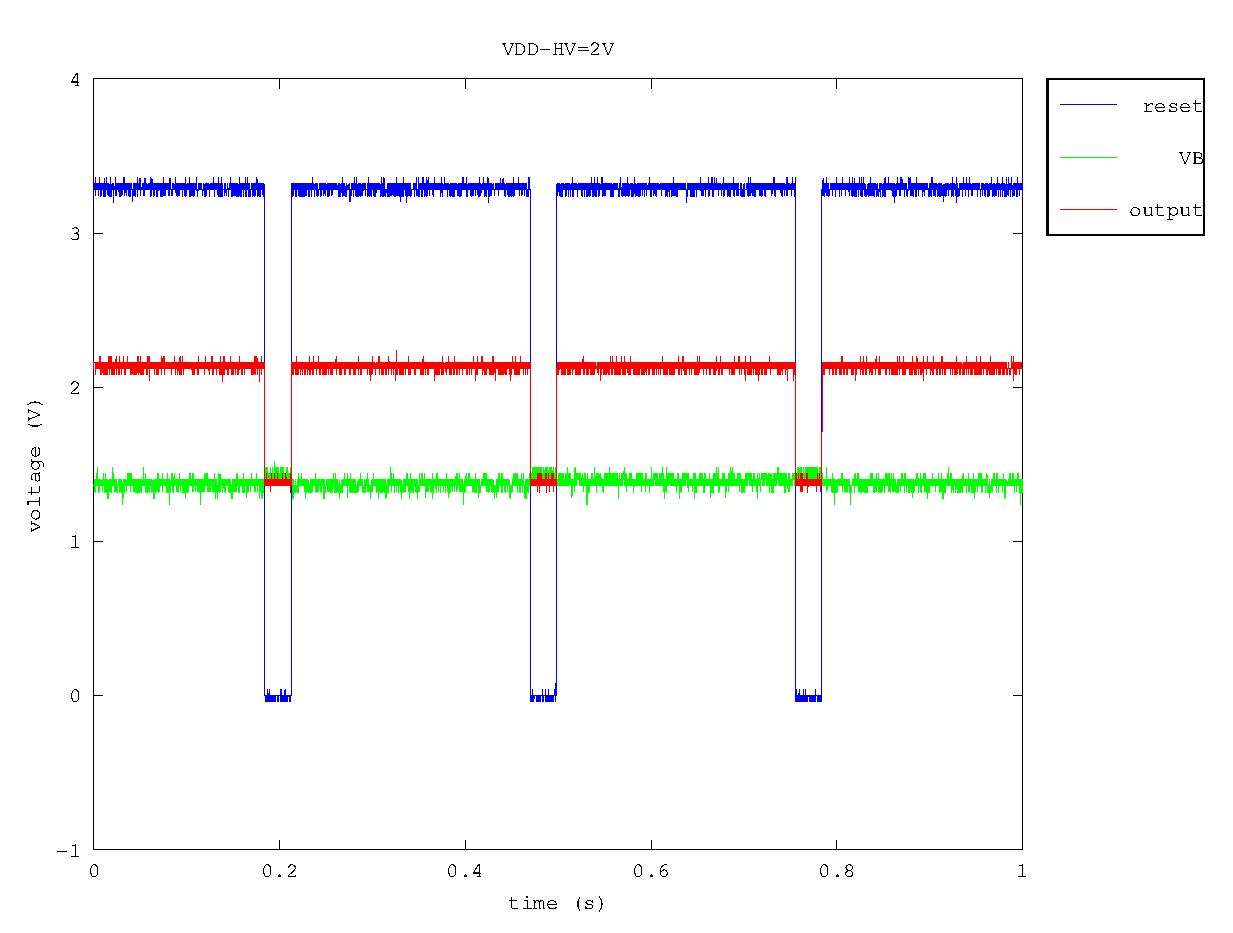
\includegraphics[width=0.8\linewidth]{fig/VB_2V.eps}
	\caption{VB and output for $VDD\_HV=2\,V$}
	\label{fig:VB_2V}
\end{figure}

\begin{figure}[H]
	\centering
	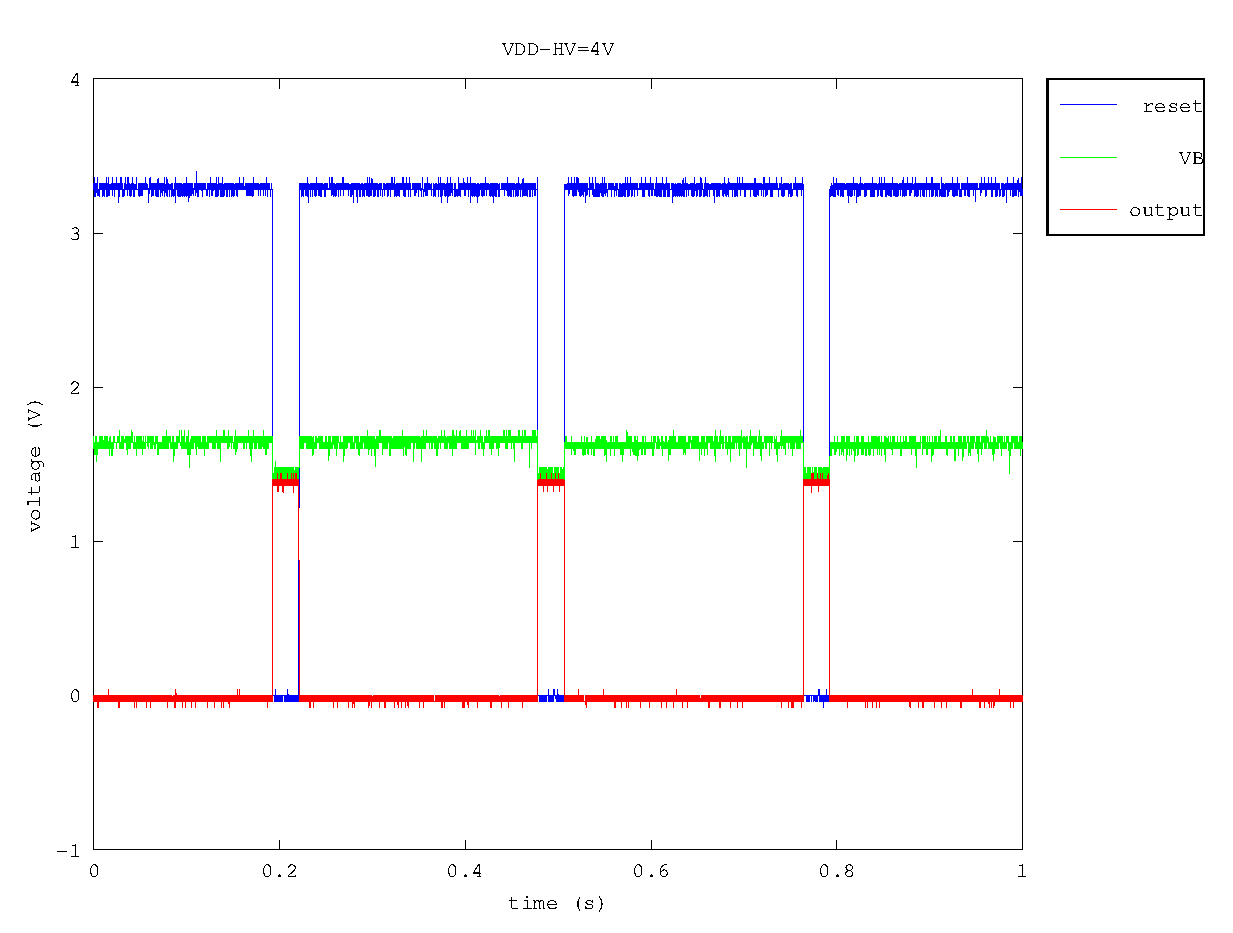
\includegraphics[width=0.8\linewidth]{fig/VB_4V.eps}
	\caption{VB and output for $VDD\_HV=4\,V$}
	\label{fig:VB_4V}
\end{figure}

\begin{figure}[H]
	\centering
	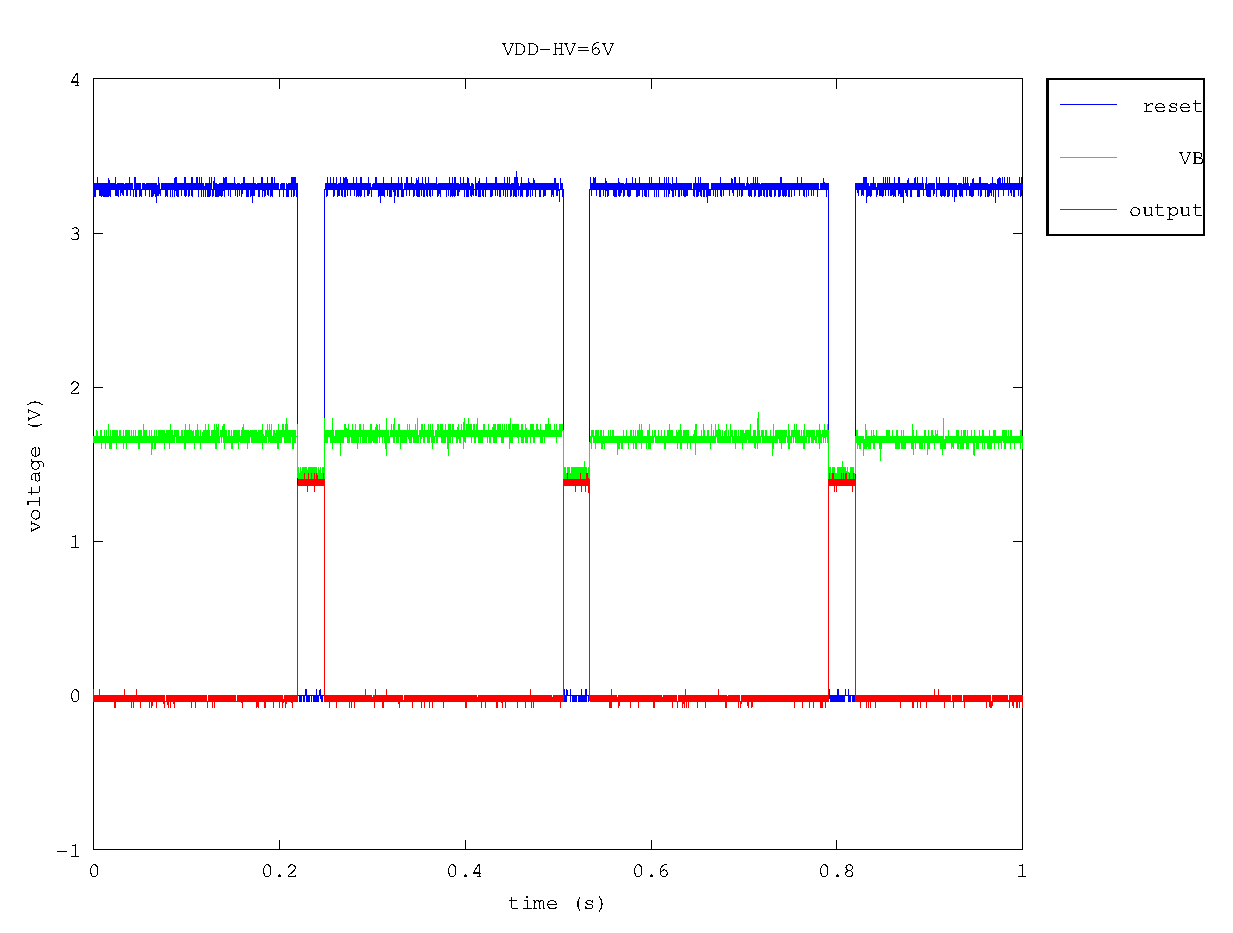
\includegraphics[width=0.8\linewidth]{fig/VB_6V.eps}
	\caption{VB and output for $VDD\_HV=6\,V$}
	\label{fig:VB_6V}
\end{figure}


\begin{figure}[H]
	\centering
	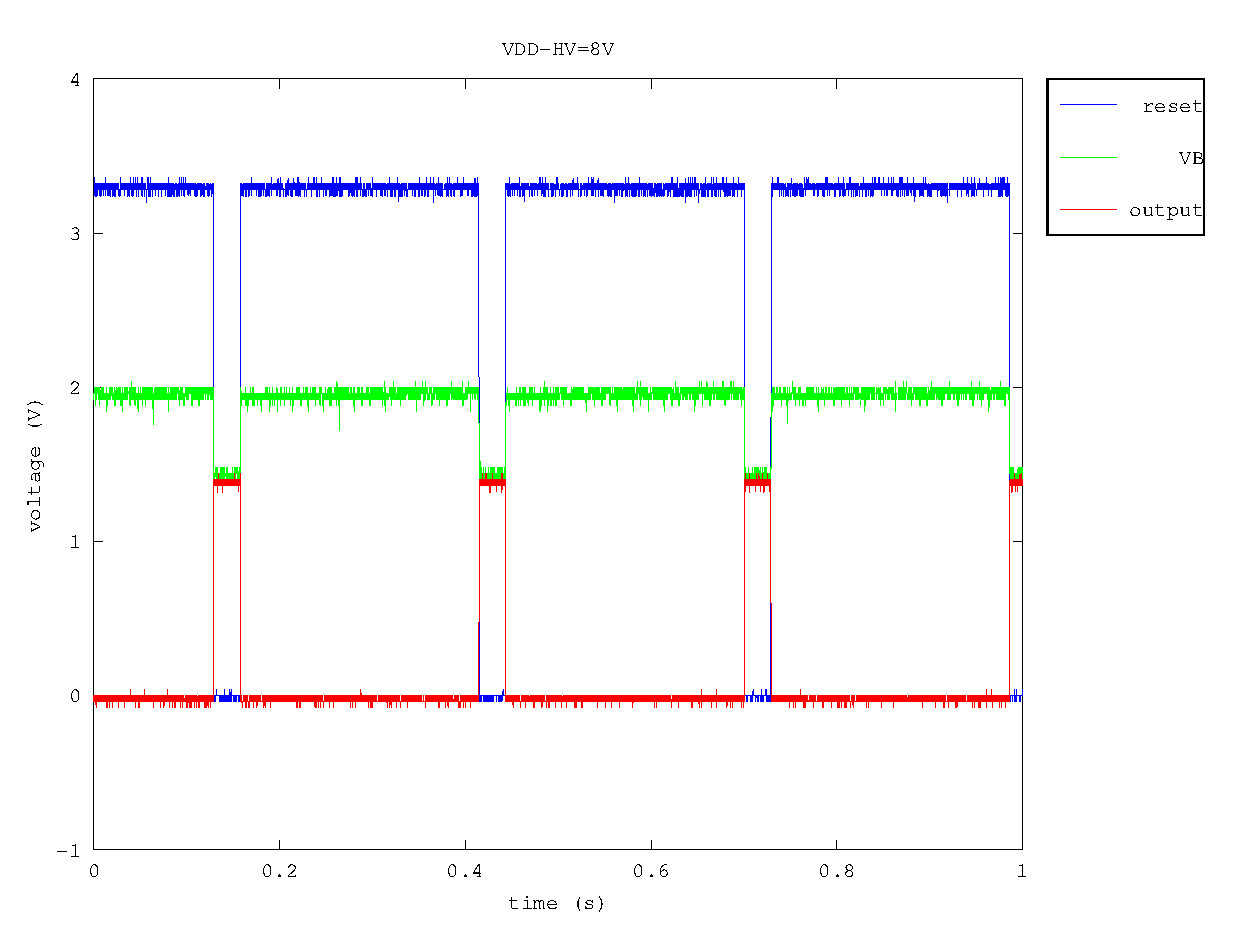
\includegraphics[width=0.8\linewidth]{fig/VB_8V.eps}
	\caption{VB and output for $VDD\_HV=8\,V$}
	\label{fig:VB_8V}
\end{figure}
\begin{figure}[H]
	\centering
	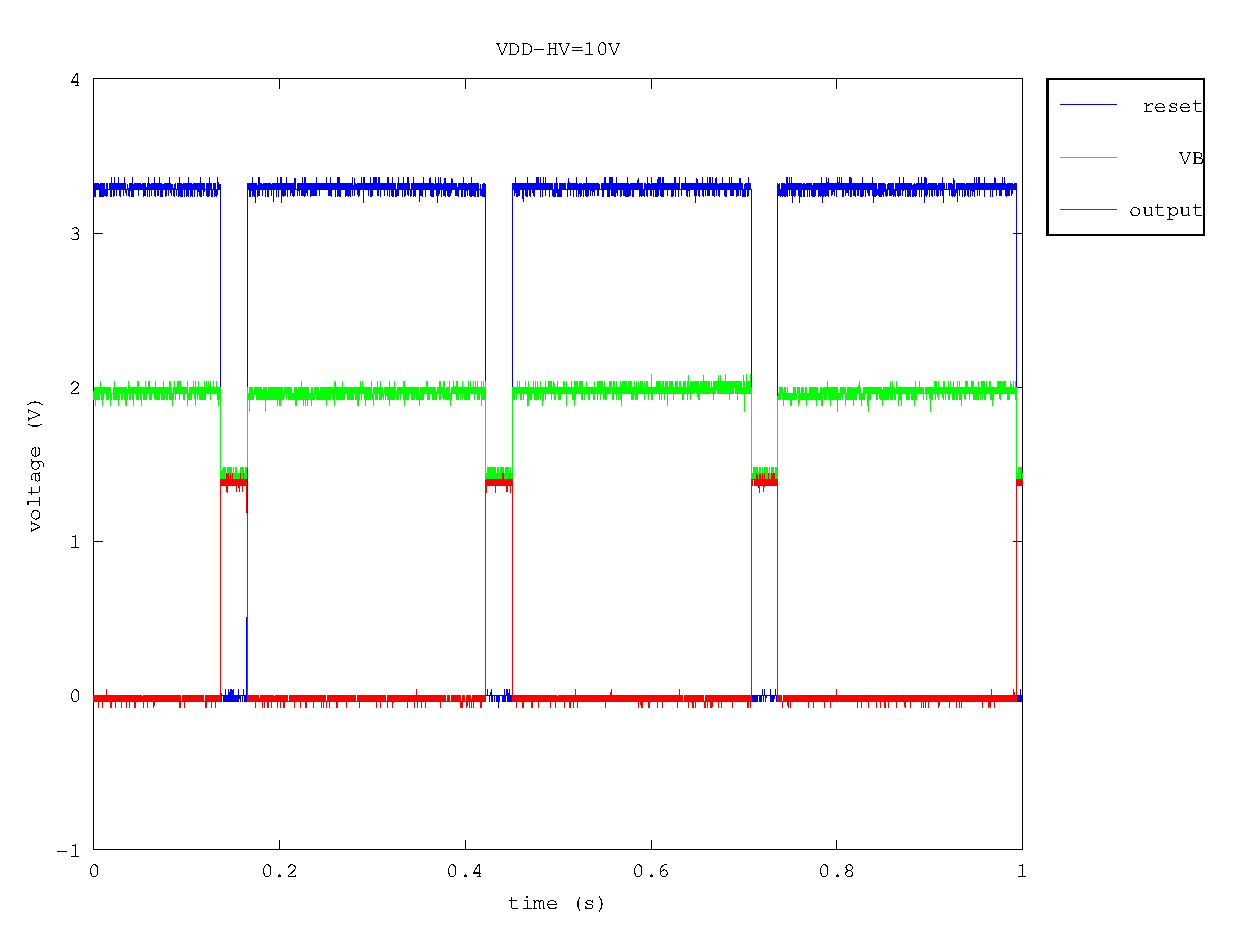
\includegraphics[width=0.8\linewidth]{fig/VB_10V.eps}
	\caption{VB and output for $VDD\_HV=10\,V$}
	\label{fig:VB_10V}
\end{figure}
\begin{figure}[H]
	\centering
	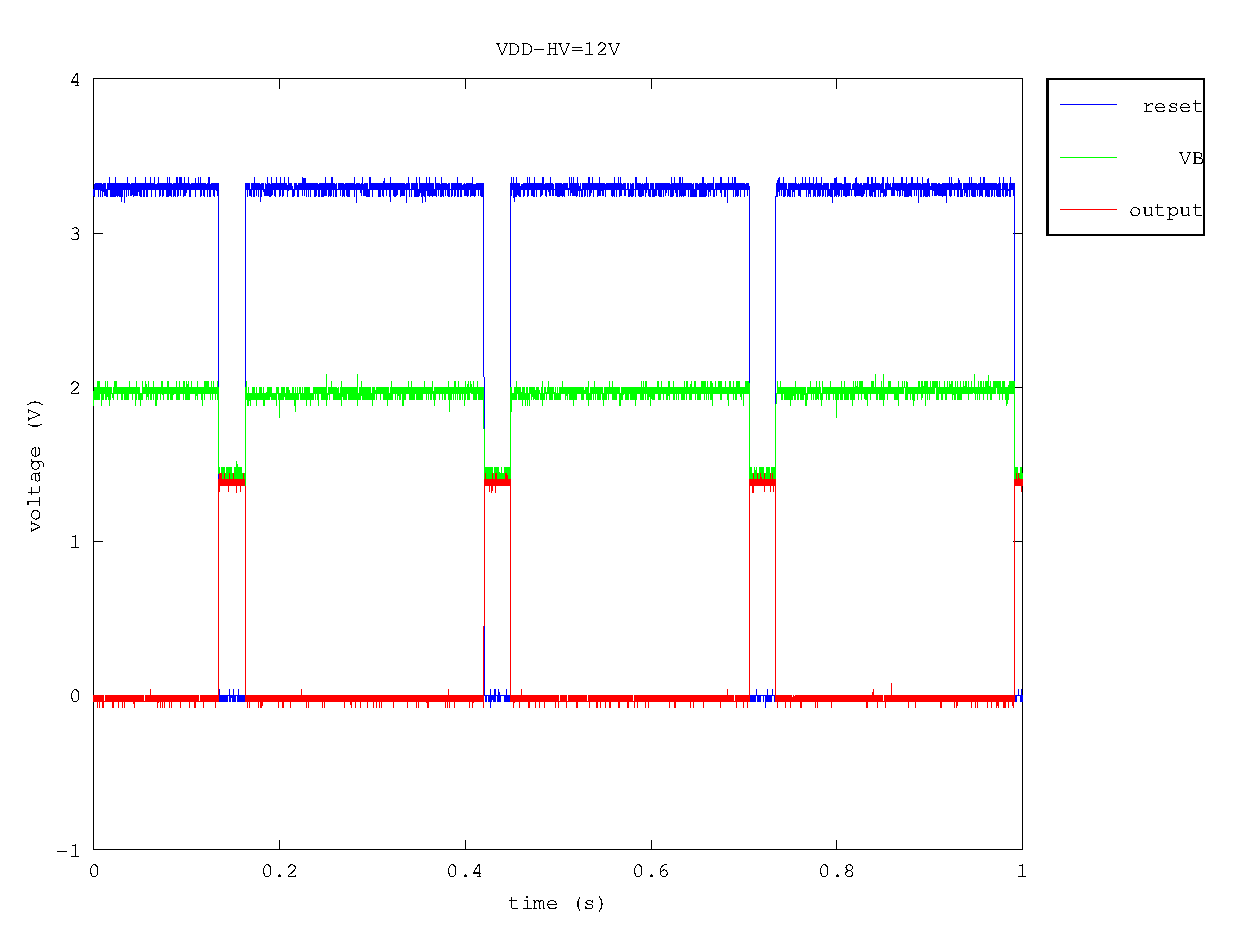
\includegraphics[width=0.8\linewidth]{fig/VB_12V.eps}
	\caption{VB and output for $VDD\_HV=12\,V$}
	\label{fig:VB_12V}
\end{figure}

\begin{figure}[H]
	\centering
	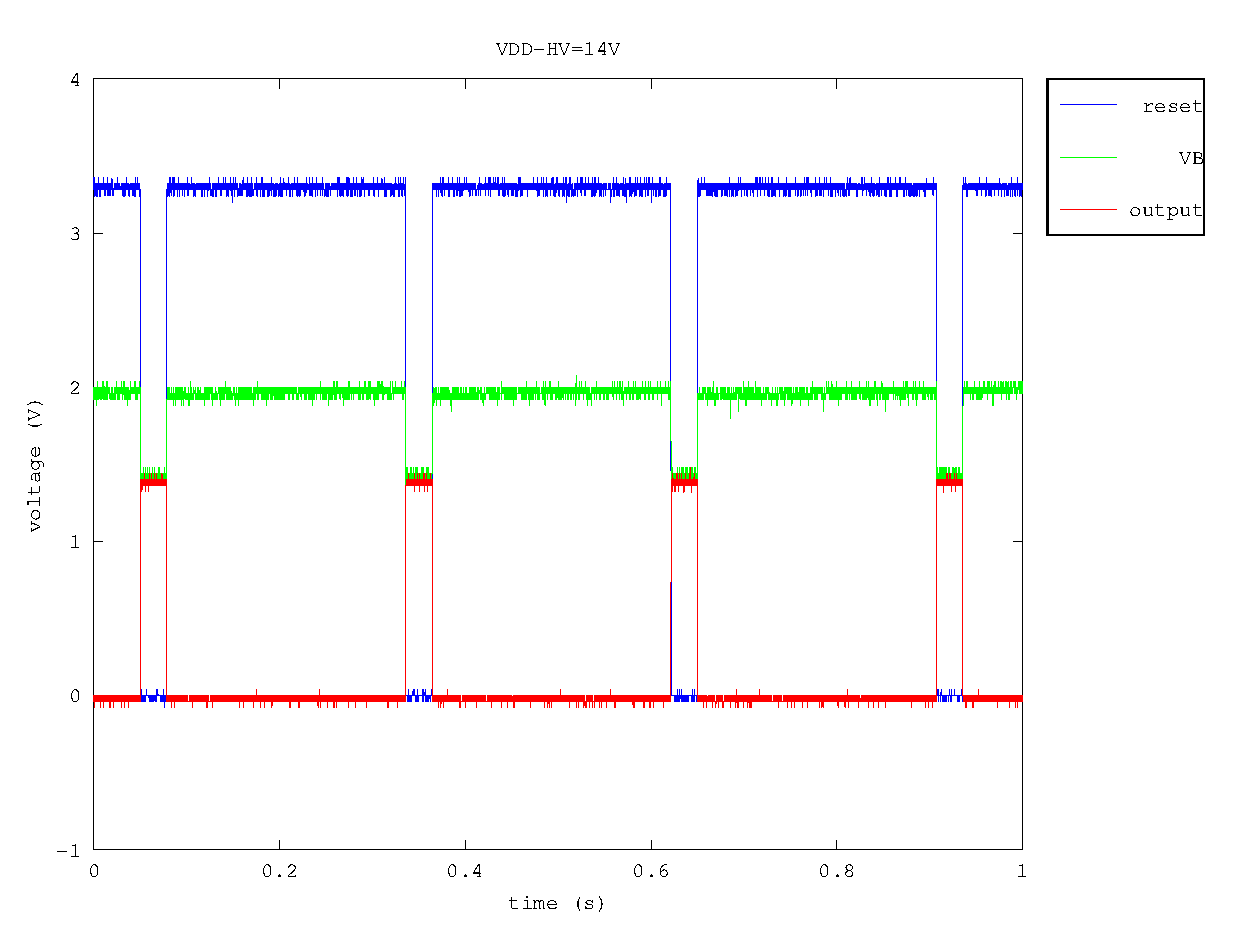
\includegraphics[width=0.8\linewidth]{fig/VB_14V.eps}
	\caption{VB and output for $VDD\_HV=14\,V$}
	\label{fig:VB_14V}
\end{figure}


\end{document}












